\documentclass[letterpaper]{beamer}

\setbeamercolor{title}{bg=blue!50!gray,fg=white}
\setbeamertemplate{section in toc}[sections numbered] 
\setbeamertemplate{caption}[numbered]
\setbeamertemplate{theorems}[numbered] 
\setbeamertemplate{itemize item}{$\bullet$}
\setbeamertemplate{navigation symbols}{}
\setbeamercolor{h1}{bg=black!80!gray,fg=white}
\setbeamertemplate{footline}[frame number]
\hypersetup{
    colorlinks=true,    % 启用颜色链接
    urlcolor=blue,       % 外部链接颜色设为红色
    linkcolor=blue,      % 内部链接（如目录）颜色设为红色
    citecolor=red       % 参考文献链接颜色设为红色
}

\usepackage{amsmath}
\usepackage{bm}
\usepackage{amssymb}
\usepackage{chngcntr}
\counterwithout{theorem}{section}
\usepackage{calligra}
\usepackage{tikz}
\usepackage{xcolor}
\usetikzlibrary{calc,intersections}
\usepackage{pgfplots}
\pgfplotsset{compat=newest}
\theoremstyle{definition}
\newtheorem{theo}{Theorem}
\newtheorem{pro}{Proposition}
\newtheorem{lem}{Lemma}
\newtheorem{cor}{Corollary}
\newtheorem{claim}{Claim}
\newtheorem{assumption}{Assumption}
\newtheorem{comparison}{Comparison}
\usepackage{pgfplots}
\pgfplotsset{compat=1.16}
\usepackage{geometry}
\usepackage{setspace}
\usepackage{graphicx}
\usepackage{subcaption}
\usepackage{caption}
\captionsetup[figure]{labelfont={bf},labelformat={default},labelsep=period,name={Figure}}
\usepackage{float}
\usepackage{graphicx}
\usepackage{ragged2e}
\justifying\let\raggedright\justifying
\usepackage{bm}
\usetheme{Singapore}

\setbeamerfont{title}{size=\Large} % 设置标题字体大小
\author{Yves Zenou, 
Junjie Zhou }
\title{Network Games Made Simple}

\institute{Presented by Sijie Wang}


\date{\today}



\begin{document}
\frame{\titlepage}
\section{Intro}

\begin{frame}{Motivation}

\begin{itemize}
    \item Most of the aforementioned peer-effect studies used the \textcolor{red}{linear-in-means} model in which each agent was linearly affected by the mean action of her reference group.
    \item In this paper, we provide a new methodology that relaxes the linearity assumption of this model.
    \item However, despite few existing network models with nonlinear
best-response functions, a
general methodology that could solve these models in a unified manner does not exist yet.
\end{itemize}

\end{frame}

\begin{frame}{Literature Review}
\begin{itemize}
    \item \textbf{Network game:} For overviews, see \cite{jackson2015games}; \cite{bramoulle2016games}.
    
    
    Specially: \cite{bramoulle2014strategic}, \cite{bourles2017altruism}.
    \item \textbf{Variational inequalities:} \cite{melo2018variational}, \cite{parise2019variational}.
    \item \textbf{Potential game:} \cite{rosenthal1973class}, \cite{slade1994does}, 
    
    \cite{monderer1996potential}, \cite{voorneveld2000best}, 
    
    \cite{dubey2006strategic}
\end{itemize}

\end{frame}

\section{Concept}
\begin{frame}{VI and Nash equilibrium}
    Given a nonempty closed convex set \( K \subseteq \mathbb{R}^m \) and a continuous mapping \( F = (F_1, \ldots, F_m)' \) from \( K \) to \( \mathbb{R}^m \), the VI problem, \( VI(K, F) \), is to determine a vector \( \mathbf{x}^* \in K \subseteq \mathbb{R}^m \), such that
\begin{equation}
\langle (\mathbf{x} - \mathbf{x}^*), F(\mathbf{x}^*) \rangle \geq 0, \quad \forall \mathbf{x} \in K,
\end{equation}
where \( \langle \cdot, \cdot \rangle \) denotes the inner product. Let \( \text{Sol}(K, F) \) denote the solution set, and \( \# \text{Sol}(K, F) \) denote the cardinality of the solutions.

\end{frame}
\begin{frame}{VI and Nash equilibrium}
\begin{definition}
A normal form game $\Gamma = (u_i,K_i)_{i \in \mathbb{N}}$ among $N = \{1, \ldots, n\}$ players is \textit{well-behaved} if:
\begin{enumerate}
    \item[(i)] the strategy space of each player $K_i$ is a closed and convex subset of $\mathbb{R}^{m_i}$;
    \item[(ii)] the payoff functions are twice continuously differentiable; and
    \item[(iii)] for each player $i$, for any $x_{-i} \in \prod_{j \neq i} K_j$, $u_i(x_i, x_{-i})$ is concave in $x_i \in K_i$.
\end{enumerate}
\end{definition}
\end{frame}

\begin{frame}


\begin{lem}\label{lem1}
    Suppose $\Gamma$ is a well-behaved game. Then \(\mathbf{x^*}=(x_1^*,...,x_n^*)\in \prod_i K_i\) is pure-strategy Nash equilibrium of \(\Gamma\) if and only if $\mathbf{x^*}$ solves 
    \[
 \begin{pmatrix}
\nabla_{x_1} u_1(\mathbf{x^*}) \\
\vdots \\
\nabla_{x_n} u_n(\mathbf{x^*})
\end{pmatrix}\cdot (\mathbf{x}-\mathbf{x^*}) \leq 0 \quad \forall \mathbf{x} \in \prod_i K_i
\]
\end{lem}  

\begin{proof}[Proof Sketch]
    \[
\nabla_{x_i} u_i(\mathbf{x^*})^{\top}(x_i-x_{i}^{*})\leq 0 \quad \forall i\in N, x_i \in K_i
\]
\[
\sum_{i\in N}\nabla_{x_i} u_i(\mathbf{x^*})^{\top}(x_i-x_{i}^{*})\leq 0 \quad \forall \mathbf{x} \in \prod_i K_i
\]
\end{proof}


    
\end{frame}

\begin{frame}{Sign equivalences}
\begin{definition}
Let \( VI(K, F) \) be sign equivalent to \( VI(K, \tilde{F}) \) on \( K \) if, for every \( i \),
\begin{align*}
    F_i(x) \leq 0 \quad &\text{if and only if} \quad \tilde{F}_i(x) \leq 0, \\
    &\forall x \in K.
\end{align*}
\end{definition}
\vspace{1em} % Adds some vertical space between the definitions
\begin{definition}
A set \( K \) is called rectangular if 
\begin{align*}
    K = \prod_{i=1}^{m} [a_i, b_i] \quad &\text{with} \quad -\infty \leq a_i < b_i \leq +\infty.
\end{align*}
\end{definition}
\end{frame}

\begin{frame}{Main Results}
   \begin{theo}\label{thm1}
    Suppose \( F \) and \( \tilde{F} \) are sign equivalent on \( K \).

\begin{enumerate}
    \item[(i)] Both VIs have the same set of solutions in \( \text{int}(K) \), the interior of \( K \), that is,
    \[
    \text{Sol}(K, F) \cap \text{int}(K) = \text{Sol}(K, \tilde{F}) \cap \text{int}(K).
    \]
    This means that if \( x^* \in \text{int}(K) \), then \( x^* \) solves \( VI(K, F) \) if and only if \( x^* \) solves \( VI(K, \tilde{F}) \).

    \item[(ii)] In addition, if \( K \) is rectangular, then, two VIs have the same solution set, that is,
    \[
    \text{Sol}(K, F) = \text{Sol}(K, \tilde{F}).
    \]
    This means that any \( x^* \in K \) that solves \( VI(K, F) \) must solve \( VI(K, \tilde{F}) \), and vice versa.
\end{enumerate}
   \end{theo}
\end{frame}
\begin{frame}{Main Results}
    \begin{theo}\label{thm2}
 Consider a network game $\Gamma^g = (u_i, G, K_i)_{i\in N}$ with $K_i = [a_i, b_i] \subseteq \mathbb{R}$ and $K = \prod_{i=1}^{n} K_i$. Assume that, for each $i$, there exists a scalar $\delta$, and some continuous functions $h_i(\cdot), s_i(\cdot)$ and $R_i(\cdot)$, such that player $i$'s optimal decision $x_i$, given each $x_{-i}$, implicitly satisfies
\[
h_i(x_i) = R_i\left( s_i(x_i) + \delta \sum_{j=1}^{n} g_{ij}x_j \right).
\]
Assume that $R_i(\cdot)$ is either strictly increasing or strictly decreasing. Then, $x^* = (x_1^*, \ldots, x_n^*)$ in $\text{int}(K)$ solves $(9)$ if and only if $x^*$ is a stationary point of $\phi(x)$, where
\[
\phi(x) := \sum_{i=1}^{n} \int_{0}^{x_i} \left[ R_i^{-1}(h_i(z_i)) - s_i(z_i) \right] dz_i - \frac{1}{2} \delta \sum_{i=1}^{n} \sum_{j=1}^{n} g_{ij}x_ix_j.
\]
The intuition behind Theorem 2 is simple. Consider a network game $\mathcal{T}^8 = (u_i, G, K_i)_{i\in N}$ for which the best-response function of each player $i$ is given by $(9)$. By inverting $R_i(\cdot)$ in $(9)$, we obtain:
\[
R_i^{-1}(h_i(x_i)) - s_i(x_i) - \delta \sum_{j=1}^{n} \gamma_{ij}x_j = 0, \quad \forall i.
\]
This is equivalent to
\[
\frac{\partial \phi}{\partial x_i}, \text{ for } \phi(x) \text{ defined in } (10)
\]
    \end{theo}
\end{frame}

\begin{frame}{Summary}
    \begin{figure}[h]
\centering
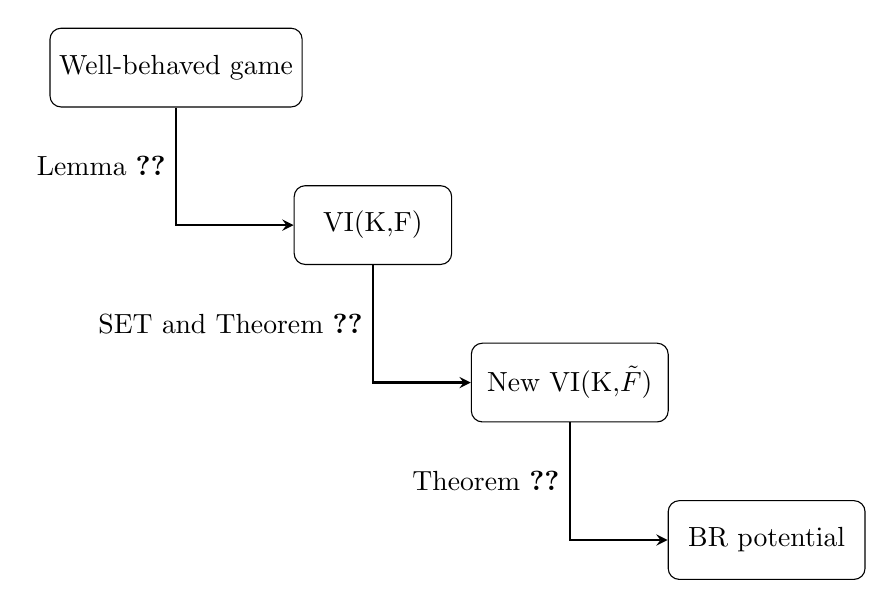
\begin{tikzpicture}[node distance=1 cm and 1 cm, auto]
    % Styles for boxes and lines
    \tikzstyle{box} = [rectangle, rounded corners, draw=black, align=center, minimum width=3cm, minimum height=1cm]
    \tikzstyle{arrow} = [thick,->,>=stealth]

  % Nodes with explicit coordinates
    \node[box][rectangle, rounded corners, draw=black, align=center, minimum width=3cm, minimum height=1cm] (wellbehaved) at (0,0) {Well-behaved game};
    \node[box][rectangle, rounded corners, draw=black, align=center, minimum width=2cm, minimum height=1cm] (VI) at (2.5,-2) {VI(K,F)};
    \node[box][rectangle, rounded corners, draw=black, align=center, minimum width=2.5cm, minimum height=1cm] (newVI) at (5,-4) {New VI(K,\(\tilde{F}\))};
    \node[box][rectangle, rounded corners, draw=black, align=center, minimum width=2.5cm, minimum height=1cm] (BR) at (7.5,-6) {BR potential};

  % Arrows with corners
    \draw[arrow] (wellbehaved) -- (wellbehaved |- VI) node[midway, left] {Lemma \ref{lem1}} -- (VI);
    \draw[arrow] (VI) -- (VI |- newVI) node[midway, left] {SET and Theorem \ref{thm1}} -- (newVI);
    \draw[arrow] (newVI) -- (newVI |- BR) node[midway, left] {Theorem \ref{thm2}} -- (BR);


\end{tikzpicture}
\end{figure}
\end{frame}

\section{Applications}

\begin{frame}{GSC in networks\cite{baetz2015social}}
\[
u_i(x, g) = v\left( \sum_{j} g_{ij}x_j \right)x_i - \frac{1}{2}x_i^2
\]
 \( v'(\cdot)>0 \),   \( v(0) = 0 \), \( v'(0) > 1 \), \( 0 \leq \lim_{x \to \infty} v'(x) < \frac{1}{n - 1} \) and \( v''(\cdot) < 0 \)

There are exactly two equilibria for any network g:
\begin{itemize}
    \item  (i) a trivial equilibrium in which all agents choose 0 and \item  (ii) a nontrivial equilibrium that is interior.
\end{itemize}
\end{frame}

\begin{frame}{GSC\cite{baetz2015social}}

\begin{figure}[h]
\centering
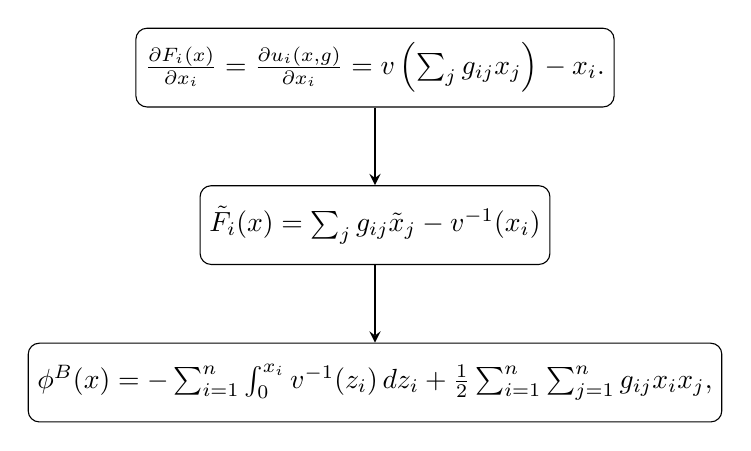
\begin{tikzpicture}[auto]
    % Styles for boxes and lines
    \tikzset{
      box/.style={rectangle, rounded corners, draw=black, align=center, minimum width=3cm, minimum height=1cm},
      arrow/.style={thick,->,>=stealth}
    }

    % Nodes with explicit coordinates
    \node[box] (VI) at (3,-1) {
$\frac{\partial F_i(x)}{\partial x_i}=\frac{\partial u_i(x, g)}{\partial x_i} =  v\left( \sum_{j} g_{ij} x_j \right)-x_i .
$};
    \node[box] (newVI)at (3,-3) {
$\tilde{F}_i(x) =  \sum_{j} g_{ij} \tilde{x}_j-v^{-1}(x_i) $};
    \node[box] (BR) at (3,-5){$\phi^B(x) = -\sum_{i=1}^{n} \int_{0}^{x_i} v^{-1}(z_i) \, dz_i + \frac{1}{2} \sum_{i=1}^{n} \sum_{j=1}^{n} g_{ij}x_i x_j,$};

    % Arrows with labels
    \draw[arrow] (VI) -- node[midway, right] {} (newVI);
    \draw[arrow] (newVI) -- node[midway, right] {} (BR);

\end{tikzpicture}
\caption{Our methodology}
\end{figure}
\end{frame}

\begin{frame}
\begin{pro}
 Suppose \( v(0) \geq 0 \), \( v'(z) > 0 \) for \( z \geq 0 \), and \(\max_{z} \{ v'(z) \} < \frac{1}{\lambda_{\text{max}}(G)}
\) holds. Then, there exists a unique equilibrium of the game \( \Gamma^B \).   
\end{pro}

\begin{comparison}
     \( v'(\cdot)>0 \),   \( v(0) = 0 \), \( v'(0) > 1 \), \( 0 \leq \lim_{x \to \infty} v'(x) < \frac{1}{n - 1} \) and \( v''(\cdot) < 0 \)

\end{comparison}
\end{frame}


\begin{frame}{GSS in networks\cite{bramoulle2007public}}
\[
u_i^{BKC}(x, g) = b(x_i + \delta \sum_{j} g_{ij}x_j) - c(x_i), \quad X=\mathbb{R}^n_+
\]
\begin{assumption}\label{assmpt1}
    \( b(\cdot) \) is strictly increasing and strictly concave, and \( c(\cdot) \) is strictly increasing and weakly convex. Standard Inada conditions: \( b'(0) > c'(0) \) and \( \lim_{x_i \rightarrow +\infty} b'(x_i) < \lim_{x_i \rightarrow +\infty} c'(x_i) \).
\end{assumption}
\end{frame}
\begin{frame}{GSS in networks\cite{bramoulle2007public}}
    \begin{figure}[h]
\centering
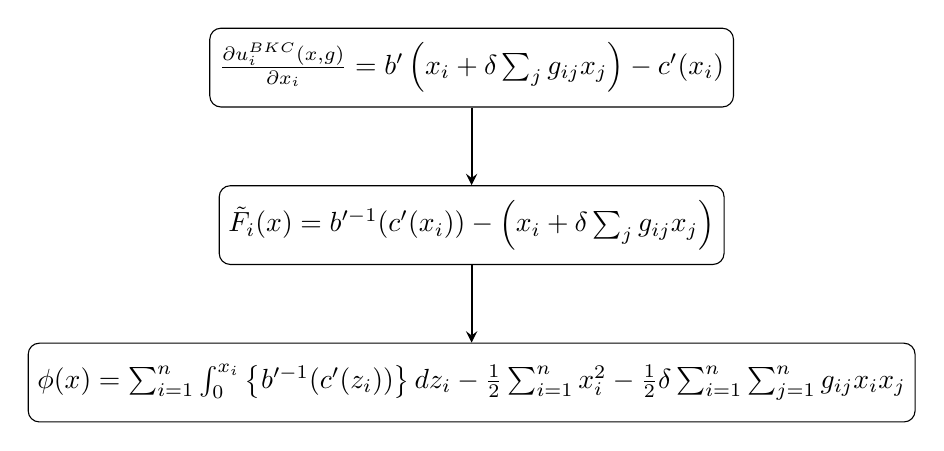
\begin{tikzpicture}[auto]
    % Styles for boxes and lines
    \tikzset{
      box/.style={rectangle, rounded corners, draw=black, align=center, minimum width=3cm, minimum height=1cm},
      arrow/.style={thick,->,>=stealth}
    }

    % Nodes with explicit coordinates
    \node[box] (VI) at (3,-1) {
$
\frac{\partial u_i^{BKC}(x, g)}{\partial x_i} = b'\left(x_i + \delta \sum_{j} g_{ij}x_j\right)-c'(x_i)$};
    \node[box] (newVI)at (3,-3) {
$\tilde{F}_i(x) =   b'^{-1}(c'(x_i))-\left(x_i + \delta \sum_{j} g_{ij}x_j\right)  $};
    
    \node[box] (BR) at (3,-5){$\phi(x) = \sum_{i=1}^{n} \int_{0}^{x_i} \left\{ b'^{-1}(c'(z_i)) \right\} dz_i - \frac{1}{2} \sum_{i=1}^{n} x_i^2 - \frac{1}{2} \delta \sum_{i=1}^{n} \sum_{j=1}^{n} g_{ij} x_i x_j$};

    % Arrows with labels
    \draw[arrow] (VI) -- node[midway, right] {} (newVI);
    \draw[arrow] (newVI) -- node[midway, right] {} (BR);

\end{tikzpicture}
\caption{Our methodology}
\end{figure}
\end{frame}

\begin{frame}{GSS in networks\cite{bramoulle2007public}}
\[\phi^{BKC}(x) = \sum_{i=1}^{n} \int_{0}^{x_i} \left\{ b'^{-1}(c'(z_i)) \right\} dz_i - \frac{1}{2} \sum_{i=1}^{n} x_i^2 - \frac{1}{2} \delta \sum_{i=1}^{n} \sum_{j=1}^{n} g_{ij} x_i x_j\]
\[
\textbf{H} \left[ \phi^{BKC}(x) \right] = \textbf{D} - (\textbf{I} + \delta \textbf{G})
\]
\begin{pro}
    Consider the network public-good game \(\Gamma^{BKC}\) and suppose that Assumption \ref{assmpt1} holds. If, in addition, \(\delta \lambda_{\min}(G) + 1 > 0\), then (i) \(\phi^{BKC}(x)\) is strictly concave and (ii) there exists a unique Nash equilibrium in \(\Gamma^{BKC}\).
\end{pro}

\end{frame}
\begin{frame}{GSS in networks\cite{bramoulle2007public}}
\begin{comparison}
     If, the autarky solution is \( k^* = b'^{-1}(1) \), then, \( \phi^{BKC}(x) \) reduces to
\[
\phi^{BK}(x) = \sum_{i} \left( k^* x_i - \frac{1}{2} x_i^2 \right) + \delta \sum_{ij} g_{ij}x_ix_j,
\]
\end{comparison}

\begin{assumption}\label{assmpt2}
    \(b^{'}(0)>c^{'}(0)=0\).
\end{assumption}

\end{frame}

\begin{frame}{GSS in networks\cite{bramoulle2007public}}
\begin{pro}
     Consider the network public-good game \(\Gamma^{BKC}\) and suppose that Assumptions \ref{assmpt1} and \ref{assmpt2} hold. In addition, assume that \(\delta = 1\). Then the following statements hold: 
\begin{itemize}
  \item[(i)] Any Nash equilibrium \(x^*\) is interior, that is, \(x^*_i > 0\), for all \(i\).
  \item[(ii)] At any Nash equilibrium \(x^*\),
  \begin{enumerate}
    \item[(a)] \(N_i \subseteq (\subset) N_j \implies x^*_i \geq (>) x^*_j\).
    \item[(b)] \(N_i \subseteq (\subset) N_j \implies x^*_i  \geq(>) x^*_j\), where \(N_i = N_j \cup \{i\}\).
  \end{enumerate}
  \item[(iii)] For the complete network, there exists a unique Nash equilibrium in which every agent exerts the same effort \(x^*\), where \(x^*\) uniquely solves \(b'(n x^*) = c'(x^*)\).
  \item[(iv)] For the star network (\(n \geq 3\)), in any Nash equilibrium, the center node exerts strictly less effort than any of the periphery nodes, while all periphery nodes exert the same effort.
\end{itemize}
\end{pro}
\end{frame}

\begin{frame}{GSS in networks\cite{bramoulle2007public}}
    \begin{comparison}
    \begin{itemize}
        \item For the complete network, \cite{bramoulle2007public} predict a specialized equilibrium in which a single node exerts \(k^*\), while all the remaining nodes free ride by choosing zero.In addition, there is a continuum of equilibria. Indeed, \((x^*_1, \ldots, x^*_n)\) is a Nash equilibrium as long as the sum of \(x^*_i\) adds up to \(k^*\). 
        \item  In the \emph{star network}, \cite{bramoulle2007public} show that only specialized profiles are equilibria and there are just two Nash equilibria: either the center or the three agents at the periphery are specialists. This implies, in particular, that the center node can exert either a higher or a lower effort than the periphery nodes. 
    \end{itemize}

    \end{comparison}
\end{frame}



\begin{frame}{Directed network games\cite{bayer2023best}}
\[
\pi_i(\mathbf{x}) = f_i \left( \sum_{j \in I} w_{ij}x_j \right) - c_i x_i,
\]
\( f^{'}_i > 0 \), \( f^{''}_i < 0 \), \( w_{ij} \in \mathbb{R} \), \( w_{ii} = 1 \), and \( c_i > 0 \) for every \( i, j \in I \).


\begin{definition}
We say that the weight matrix \( W \) shows \textit{transitive relative importance} if for every \( 3 \leq m \leq n \) and for all pairwise distinct \( i_1, i_2, \ldots, i_m \in I \) we have
\[
w_{i_1 i_2} w_{i_2 i_3} \cdots w_{i_{m-1} i_m} w_{i_m i_1} = w_{i_1 i_m} w_{i_m i_{m-1}} \cdots w_{i_3 i_2} w_{i_2 i_1}.
\]
\end{definition}
\end{frame}

\begin{frame}{Directed network games\cite{bayer2023best}}
    \begin{definition}
We say that the weight matrix \( W \) is sign-symmetric if for every \(\{i, j\} \subseteq I\) we have \(\text{sgn}(w_{ij}) = \text{sgn}(w_{ji})\).
    \end{definition}
\begin{theo}
 The following statements are equivalent:
\begin{enumerate}
    \item \( W \) is rescalable into a symmetric matrix,
    \item \( W \) is transitive and sign-symmetric,
    \item there exists a game \( G \) on \( W \) that has a quadratic best-response potential function,
    \item every game \( G \) on \( W \) has a quadratic best-response potential function.
\end{enumerate}

\end{theo}
\end{frame}


\begin{frame}{Directed network games\cite{bayer2023best}}
    \begin{figure}[h]
\centering
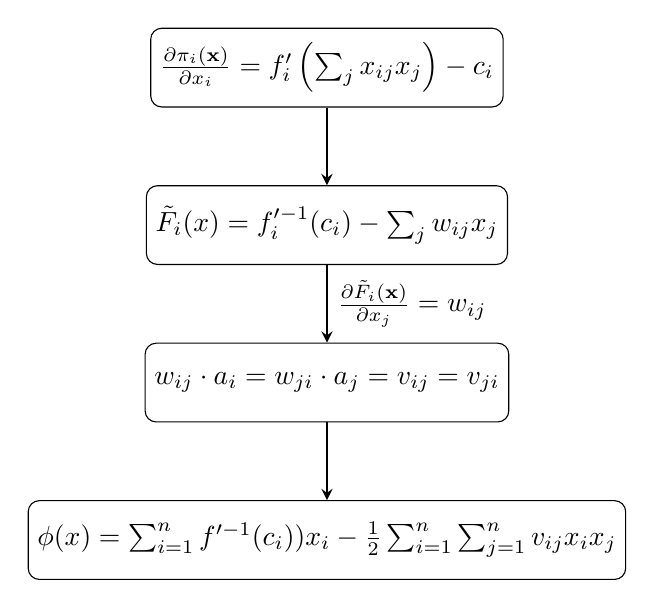
\begin{tikzpicture}[auto]
    % Styles for boxes and lines
    \tikzset{
      box/.style={rectangle, rounded corners, draw=black, align=center, minimum width=3cm, minimum height=1cm},
      arrow/.style={thick,->,>=stealth}
    }

    % Nodes with explicit coordinates
    \node[box] (VI) at (3,-1) {
$
\frac{\partial \pi_i(\textbf{x})}{\partial x_i} = f_{i}'\left(\sum_{j} x_{ij}x_j\right)-c_i$};
    \node[box] (newVI)at (3,-3) {
$\Tilde{F}_i(x) =  f_{i}'^{-1}(c_i)- \sum_{j} w_{ij}x_j  $};
    
    \node[box] (BR) at (3,-5){$w_{ij}\cdot a_i=w_{ji}\cdot a_j=v_{ij}=v_{ji}$};
    \node[box] (VV) at (3,-7){$\phi(x) = \sum_{i=1}^{n}  f'^{-1}(c_i))x_i - \frac{1}{2}  \sum_{i=1}^{n} \sum_{j=1}^{n} v_{ij} x_i x_j$};

    % Arrows with labels
    \draw[arrow] (VI) -- node[midway, right] {} (newVI);
    \draw[arrow] (newVI) -- node[midway, right] {\(\frac{\partial \tilde{F}_i(\textbf{x})}{\partial x_j}=w_{ij}\)} (BR);
    \draw[arrow] (BR) -- node[midway, right] {} (VV);

\end{tikzpicture}
\caption{Our methodology}
\end{figure}
\end{frame}




















\section{Acknowledgements}
\begin{frame}{}
\begin{tikzpicture}[overlay, remember picture]
\node at (current page.center) {
  \fontsize{48}{56}\selectfont
  \calligra
  Thank You!
};
\end{tikzpicture}
\end{frame}


\newpage
\bibliographystyle{apalike}
\bibliography{ref} 
\end{document} 
